% !TEX root = main.tex

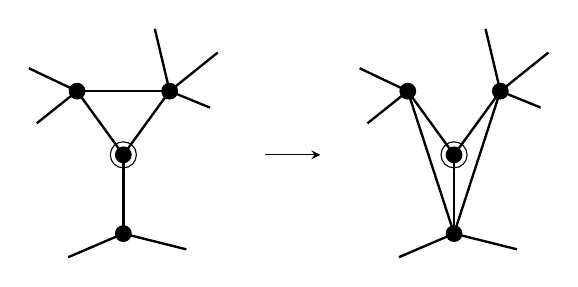
\begin{tikzpicture}

\node[circle, fill=black, draw, scale=0.6] (1) at ({sin(0*360/5)}, {-cos(0*360/5)}){};
% \node[circle, fill=black, draw, scale=0.6] (2) at ({sin(1*360/5)}, {cos(1*360/5)}){};
\node[circle, fill=black, draw, scale=0.6] (3) at ({sin(2*360/5)}, {-cos(2*360/5)}){};
\node[circle, fill=black, draw, scale=0.6] (4) at ({sin(3*360/5)}, {-cos(3*360/5)}){};
% \node[circle, fill=black, draw, scale=0.6] (5) at ({sin(4*360/5)}, {cos(4*360/5)}){};

\node[circle, fill=white, draw, scale=1] (0) at (0.0, -0){};
\node[circle, fill=black, draw, scale=0.6] (0) at (0.0, -0){};

% \node[diamond, fill=black, draw, scale=0.6] (d2) at (-0.6, 2.5){};



% \node[scale=1] (1l) at (0, 1*1.3){$1$};
% \node[scale=1] (2l) at ({sin(1*360/5)*1.3}, {cos(1*360/5)*1.3}){$2$};
% \node[scale=1] (3l) at ({sin(2*360/5)*1.3}, {cos(2*360/5)*1.3}){$3$};
% \node[scale=1] (4l) at ({sin(3*360/5)*1.3}, {cos(3*360/5)*1.3}){$4$};
% \node[scale=1] (5l) at ({sin(4*360/5)*1.3}, {cos(4*360/5)*1.3}){$5$};

% \node[scale=1] (0) at (0, 0){$5$};

\draw[line width = 0.3mm] ({sin(2*360/5)}, {-cos(2*360/5)}) -- ({sin(3*360/5)}, {-cos(3*360/5)});

\draw[line width = 0.3mm] (0,-1) -- (0.8, -1.2);
\draw[line width = 0.3mm] (0,-1) -- (-0.7, -1.3);

\draw[line width = 0.3mm] ({sin(2*360/5)}, {-cos(2*360/5)}) -- (1.1, 0.6);
\draw[line width = 0.3mm] ({sin(2*360/5)}, {-cos(2*360/5)}) -- (1.2, 1.3);
\draw[line width = 0.3mm] ({sin(2*360/5)}, {-cos(2*360/5)}) -- (0.4, 1.6);
\draw[line width = 0.3mm] ({sin(3*360/5)}, {-cos(3*360/5)}) -- (-1.1, 0.4);
\draw[line width = 0.3mm] ({sin(3*360/5)}, {-cos(3*360/5)}) -- (-1.2, 1.1);


\draw[line width = 0.3mm] (0,-1) -- (0, -0);
% \draw[line width = 0.3mm] ({sin(1*360/5)}, {cos(1*360/5)}) -- (0, 0);
\draw[line width = 0.3mm] ({sin(2*360/5)}, {-cos(2*360/5)}) -- (0, -0);
\draw[line width = 0.3mm] ({sin(3*360/5)}, {-cos(3*360/5)}) -- (0, -0);
% \draw[line width = 0.3mm] ({sin(4*360/5)}, {cos(4*360/5)}) -- (0, 0);


% \draw[line width = 0.3mm] (-0.6, 2.5) -- (-1,1);
% \draw[line width = 0.3mm] (-0.6, 2.5) -- (1,-1);
% \draw[line width = 0.3mm] (-0.6, 2.5) -- (1,1);

% \draw[line width = 0.3mm] (0.6, 2.5) -- (-1,-1);
% \draw[line width = 0.3mm] (0.6, 2.5) -- (1,-1);

% \draw[line width = 0.3mm] (0.6, 2.5) -- (-0.6,2.5);

% \draw[line width = 0.3mm] (-1,+1) -- (+1,+1) -- (+1,-1) -- (-1,-1) -- (-1, +1);
% \draw[line width = 0.3mm] (-1,+1) -- (+1,-1);

\draw [-stealth](1.8, 0) -- (2.5,0);




%%%%%%%%%%%%%%%%%%%%%%%%%%%%%


%%%%%%%%%%%%%%%%%%%%%%%%%%%%%%%%%%

\def\ra{4.2}


\node[circle, fill=black, draw, scale=0.6] (1) at ({sin(0*360/5)+\ra}, {-cos(0*360/5)}){};
% \node[circle, fill=black, draw, scale=0.6] (2) at ({sin(1*360/5)}, {cos(1*360/5)}){};
\node[circle, fill=black, draw, scale=0.6] (3) at ({sin(2*360/5)+\ra}, {-cos(2*360/5)}){};
\node[circle, fill=black, draw, scale=0.6] (4) at ({sin(3*360/5)+\ra}, {-cos(3*360/5)}){};
% \node[circle, fill=black, draw, scale=0.6] (5) at ({sin(4*360/5)}, {cos(4*360/5)}){};

\node[circle, fill=white, draw, scale=1] (0) at (0.0+\ra, -0){};
\node[circle, fill=black, draw, scale=0.6] (0) at (0.0+\ra, -0){};

% \node[diamond, fill=black, draw, scale=0.6] (d2) at (-0.6, 2.5){};



% \node[scale=1] (1l) at (0, 1*1.3){$1$};
% \node[scale=1] (2l) at ({sin(1*360/5)*1.3}, {cos(1*360/5)*1.3}){$2$};
% \node[scale=1] (3l) at ({sin(2*360/5)*1.3}, {cos(2*360/5)*1.3}){$3$};
% \node[scale=1] (4l) at ({sin(3*360/5)*1.3}, {cos(3*360/5)*1.3}){$4$};
% \node[scale=1] (5l) at ({sin(4*360/5)*1.3}, {cos(4*360/5)*1.3}){$5$};

% \node[scale=1] (0) at (0, 0){$5$};

% \draw[line width = 0.3mm] ({sin(2*360/5)+\ra}, {-cos(2*360/5)}) -- ({sin(3*360/5)+\ra}, {-cos(3*360/5)});

% \draw[line width = 0.3mm] ({sin(2*360/5)+\ra}, {-cos(2*360/5)}) -- ({sin(3*360/5)+\ra}, {-cos(3*360/5)});

\draw[line width = 0.3mm] ({sin(2*360/5)+\ra}, {-cos(2*360/5)}) -- ({0+\ra}, {-1});
\draw[line width = 0.3mm] ({sin(3*360/5)+\ra}, {-cos(3*360/5)}) -- ({0+\ra}, {-1});


% \draw[line width = 0.3mm] ({0+\ra}, {-1, ) -- ({sin(3*360/5)+\ra}, {-cos(3*360/5)});

\draw[line width = 0.3mm] (0+\ra,-1) -- (0.8+\ra, -1.2);
\draw[line width = 0.3mm] (0+\ra,-1) -- (-0.7+\ra, -1.3);

\draw[line width = 0.3mm] ({sin(2*360/5)+\ra}, {-cos(2*360/5)}) -- (1.1+\ra, 0.6);
\draw[line width = 0.3mm] ({sin(2*360/5)+\ra}, {-cos(2*360/5)}) -- (1.2+\ra, 1.3);
\draw[line width = 0.3mm] ({sin(2*360/5)+\ra}, {-cos(2*360/5)}) -- (0.4+\ra, 1.6);
\draw[line width = 0.3mm] ({sin(3*360/5)+\ra}, {-cos(3*360/5)}) -- (-1.1+\ra, 0.4);
\draw[line width = 0.3mm] ({sin(3*360/5)+\ra}, {-cos(3*360/5)}) -- (-1.2+\ra, 1.1);


\draw[line width = 0.3mm] (0+\ra,-1) -- (0+\ra, -0);
% \draw[line width = 0.3mm] ({sin(1*360/5)}, {cos(1*360/5)}) -- (0, 0);
\draw[line width = 0.3mm] ({sin(2*360/5)+\ra}, {-cos(2*360/5)}) -- (0+\ra, -0);
\draw[line width = 0.3mm] ({sin(3*360/5)+\ra}, {-cos(3*360/5)}) -- (0+\ra, -0);
% \draw[line width = 0.3mm] ({sin(4*360/5)}, {cos(4*360/5)}) -- (0, 0);





\end{tikzpicture}